\documentclass[12pt, twoside]{article}
\usepackage[letterpaper, margin=1in, headsep=0.5in]{geometry}
\usepackage[english]{babel}
\usepackage[utf8]{inputenc}
\usepackage{amsmath}
\usepackage{amsfonts}
\usepackage{amssymb}
\usepackage{tikz}
\usetikzlibrary{quotes, angles}
\usepackage{graphicx}
\usepackage{enumitem}
\usepackage{multicol}

\newif\ifmeta
\metatrue %print standards and topics tags

\title{IB Math Applications and Interpretations}
\author{Chris Huson}
\date{March 2022}

\usepackage{fancyhdr}
\pagestyle{fancy}
\fancyhf{}
\renewcommand{\headrulewidth}{0pt} % disable the underline of the header
\raggedbottom

\fancyhead[LE]{\thepage}
\fancyhead[RO]{\thepage \\ Name: \hspace{4cm} \,\\}
\fancyhead[LO]{BECA / IB Math 6 Geometry \\* 22 March 2022}

\begin{document}
\subsubsection*{6.4 Do Now Quiz: Right triangle trigonometry}
Do Now (PreQuiz)
\begin{enumerate}
\item Calculate each value. Round to the nearest thousandth.
  \begin{enumerate}
    \begin{multicols}{2}
    \item $\displaystyle \sin 11^\circ$ \vspace{1cm}
    \item $\displaystyle \cos 62^\circ$
    \item $\displaystyle \tan 23^\circ$ \vspace{1cm}
    \item $\displaystyle \sin 81^\circ$
    \end{multicols}
  \end{enumerate}
  \vspace{1cm}

\item Find $\theta$. Round to the nearest whole degree.
  \begin{enumerate}
    \begin{multicols}{2}
    \item $\displaystyle \theta = \sin^{-1} (\frac{3}{5})$ \vspace{1cm}
    \item $\displaystyle \theta = \tan^{-1} (0.88)$
    \item $\displaystyle \theta = \cos^{-1} (0.500)$ \vspace{1cm}
    \item $\displaystyle \tan \theta = \frac{11.3}{6.9}$
    \end{multicols}
  \end{enumerate} \vspace{2cm}

\item Solve each equation for $x$, rounding to the nearest tenth.
  \begin{enumerate}
    \begin{multicols}{2}
    \item $\displaystyle \cos 71^\circ = \frac{x}{15}$ \vspace{5cm}
    \item $\displaystyle \tan 49^\circ = \frac{12.7}{x}$
    \end{multicols}
  \end{enumerate}
  \vspace{3cm}

\item Given right $\triangle ABC$ with $AC=6$, $m\angle A=50^\circ$. Find the value of $BC=x$.
  \begin{flushright}
    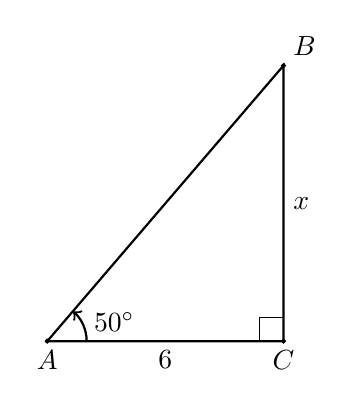
\begin{tikzpicture}[scale=0.5]
      \draw [thick](0,0)--(6,0)--(6,7)--cycle;
      \draw [fill] (0,0) circle [radius=0.05] node[below]{$A$};
      \draw [fill] (6,0) circle [radius=0.05] node[below]{$C$};
      \draw [fill] (6,7) circle [radius=0.05] node[above right]{$B$};
      \draw (6,0)++(-0.6,0)--++(0,0.6)--+(0.6,0);
      \node at (3,0)[below]{$6$};
      \node at (6,3.5)[right]{$x$};
      \draw [thick, ->] (1,0) arc [start angle=0, end angle=49, radius=1];
      \node at (1.7,0)[above]{$50^\circ$};
    \end{tikzpicture}
  \end{flushright}

\newpage
\item $\triangle ABC$ is shown with $m\angle C=90^\circ$ and the lengths of the triangle's sides are $AC=4$, $BC=7$.  \hfill (not drawn to scale)
  \begin{multicols}{2}
    \begin{enumerate}
      \item Write down the value of $\tan A$. \vspace{1.25cm}
      \item Find the measure of $\angle A$. \vspace{1cm}
      \item Write down the value of $\tan B$. \vspace{1.25cm}
      \item Find the measure of $\angle B$. \vspace{1cm}
    \end{enumerate}
    \begin{flushright}
    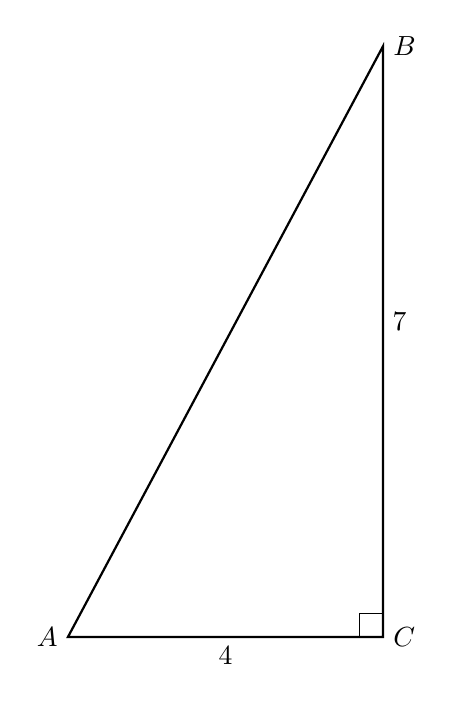
\begin{tikzpicture}[scale=0.5]
      \draw [thick]
      (0,0)node[left]{$A$}--
      (8,0)node[ right]{$C$}--
      (8,15)node[right]{$B$}--cycle;
      \draw (8,0)++(-0.6,0)--++(0,0.6)--+(0.6,0);
      \node at (4,0)[below]{$4$};
      \node at (8,8)[right]{$7$};
      %\node at (2.5,6)[above]{$17$};
    \end{tikzpicture}
    \end{flushright}
  \end{multicols}
  \vspace{2cm}
  
\item Given $\triangle ABC$ with $AC=9$ centimeters, altitude $h=7$ cm, and the base $\hat{B} = 40^\circ$. (diagram not to scale)
\begin{multicols}{2}
  \begin{enumerate}
    \item Find $\hat{A}$ using $\displaystyle \hat{A}=\sin^{-1} \frac{7}{9}$.
    \item Find $BC$ by solving the Law of Sines\\[0.5cm]
    $\displaystyle \frac{BC}{\sin A} = \frac{9}{\sin B} $
  \end{enumerate}
  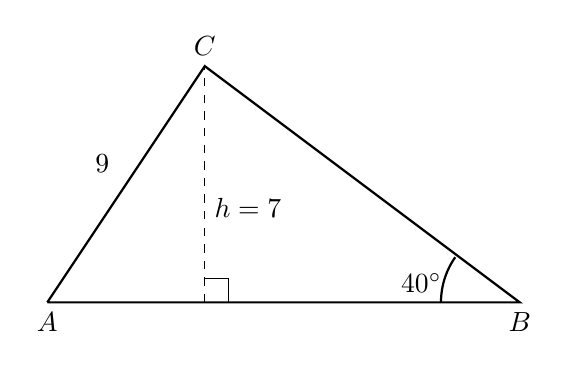
\begin{tikzpicture}[scale=1]
    \draw [thick]
      (2,0)node[below]{$A$}--
      (8,0)node[below]{$B$}--
      (4,3)node[above]{$C$} --(2,0);
    \draw [dashed] (4,0)--(4,3);
    \draw (4,0)++(0.3,0)--++(0,0.3)--+(-0.3,0);
    \node at (4,1.2)[right]{$h=7$};
    \node at (2.7,2)[below]{$9$};
    \draw [thick, -] (7,0) arc [start angle=180, end angle=145, radius=1];
    \node at (6.75,0)[above]{$40^\circ$};
    %\node at (5,0)[below]{$13 \frac{1}{2}$ cm};
  \end{tikzpicture}  
\end{multicols}
\vspace{1cm}

\end{enumerate}
\end{document}
